
To properly evaluate practical downstream metrics described in section \ref{section:model-evaluation} on model predictions, one need to be able to segment nuclei from fluorescence (as well as from predictions) first. By segmentation here the creation of mask is understood. It should constist of $0$s and $1$s, with $1$ assigned to pixels that are part of nucleus and $0$ otherwise. Altough this might be a straight-forward task for our eyes, it is not that easy to select separate nuclei via post-processing. There are several edge cases where the nuclei are difficult to segment.

Even though the most extreme corruptions mentioned in section \ref{section:nuclei-preprocessing} were filtered out, some of the images that are corrupted not that severely (meaning they still have all the visible features needed for learning) are still present in the dataset. This allow to not reduce the amount of data  significantly. The examples of difficult for segmentation cases are shown in Figure \ref{fig:lightning_conditions}.
\begin{figure}[H]
    \centering
    \setkeys{Gin}{width=\linewidth}
    \centering
        \begin{tabularx}{\textwidth}{YYYY}
            \textbf{Too few cells} &
            \textbf{Overexposure} &
            \textbf{Light gradient} &
            \textbf{Normal lightning} \\
            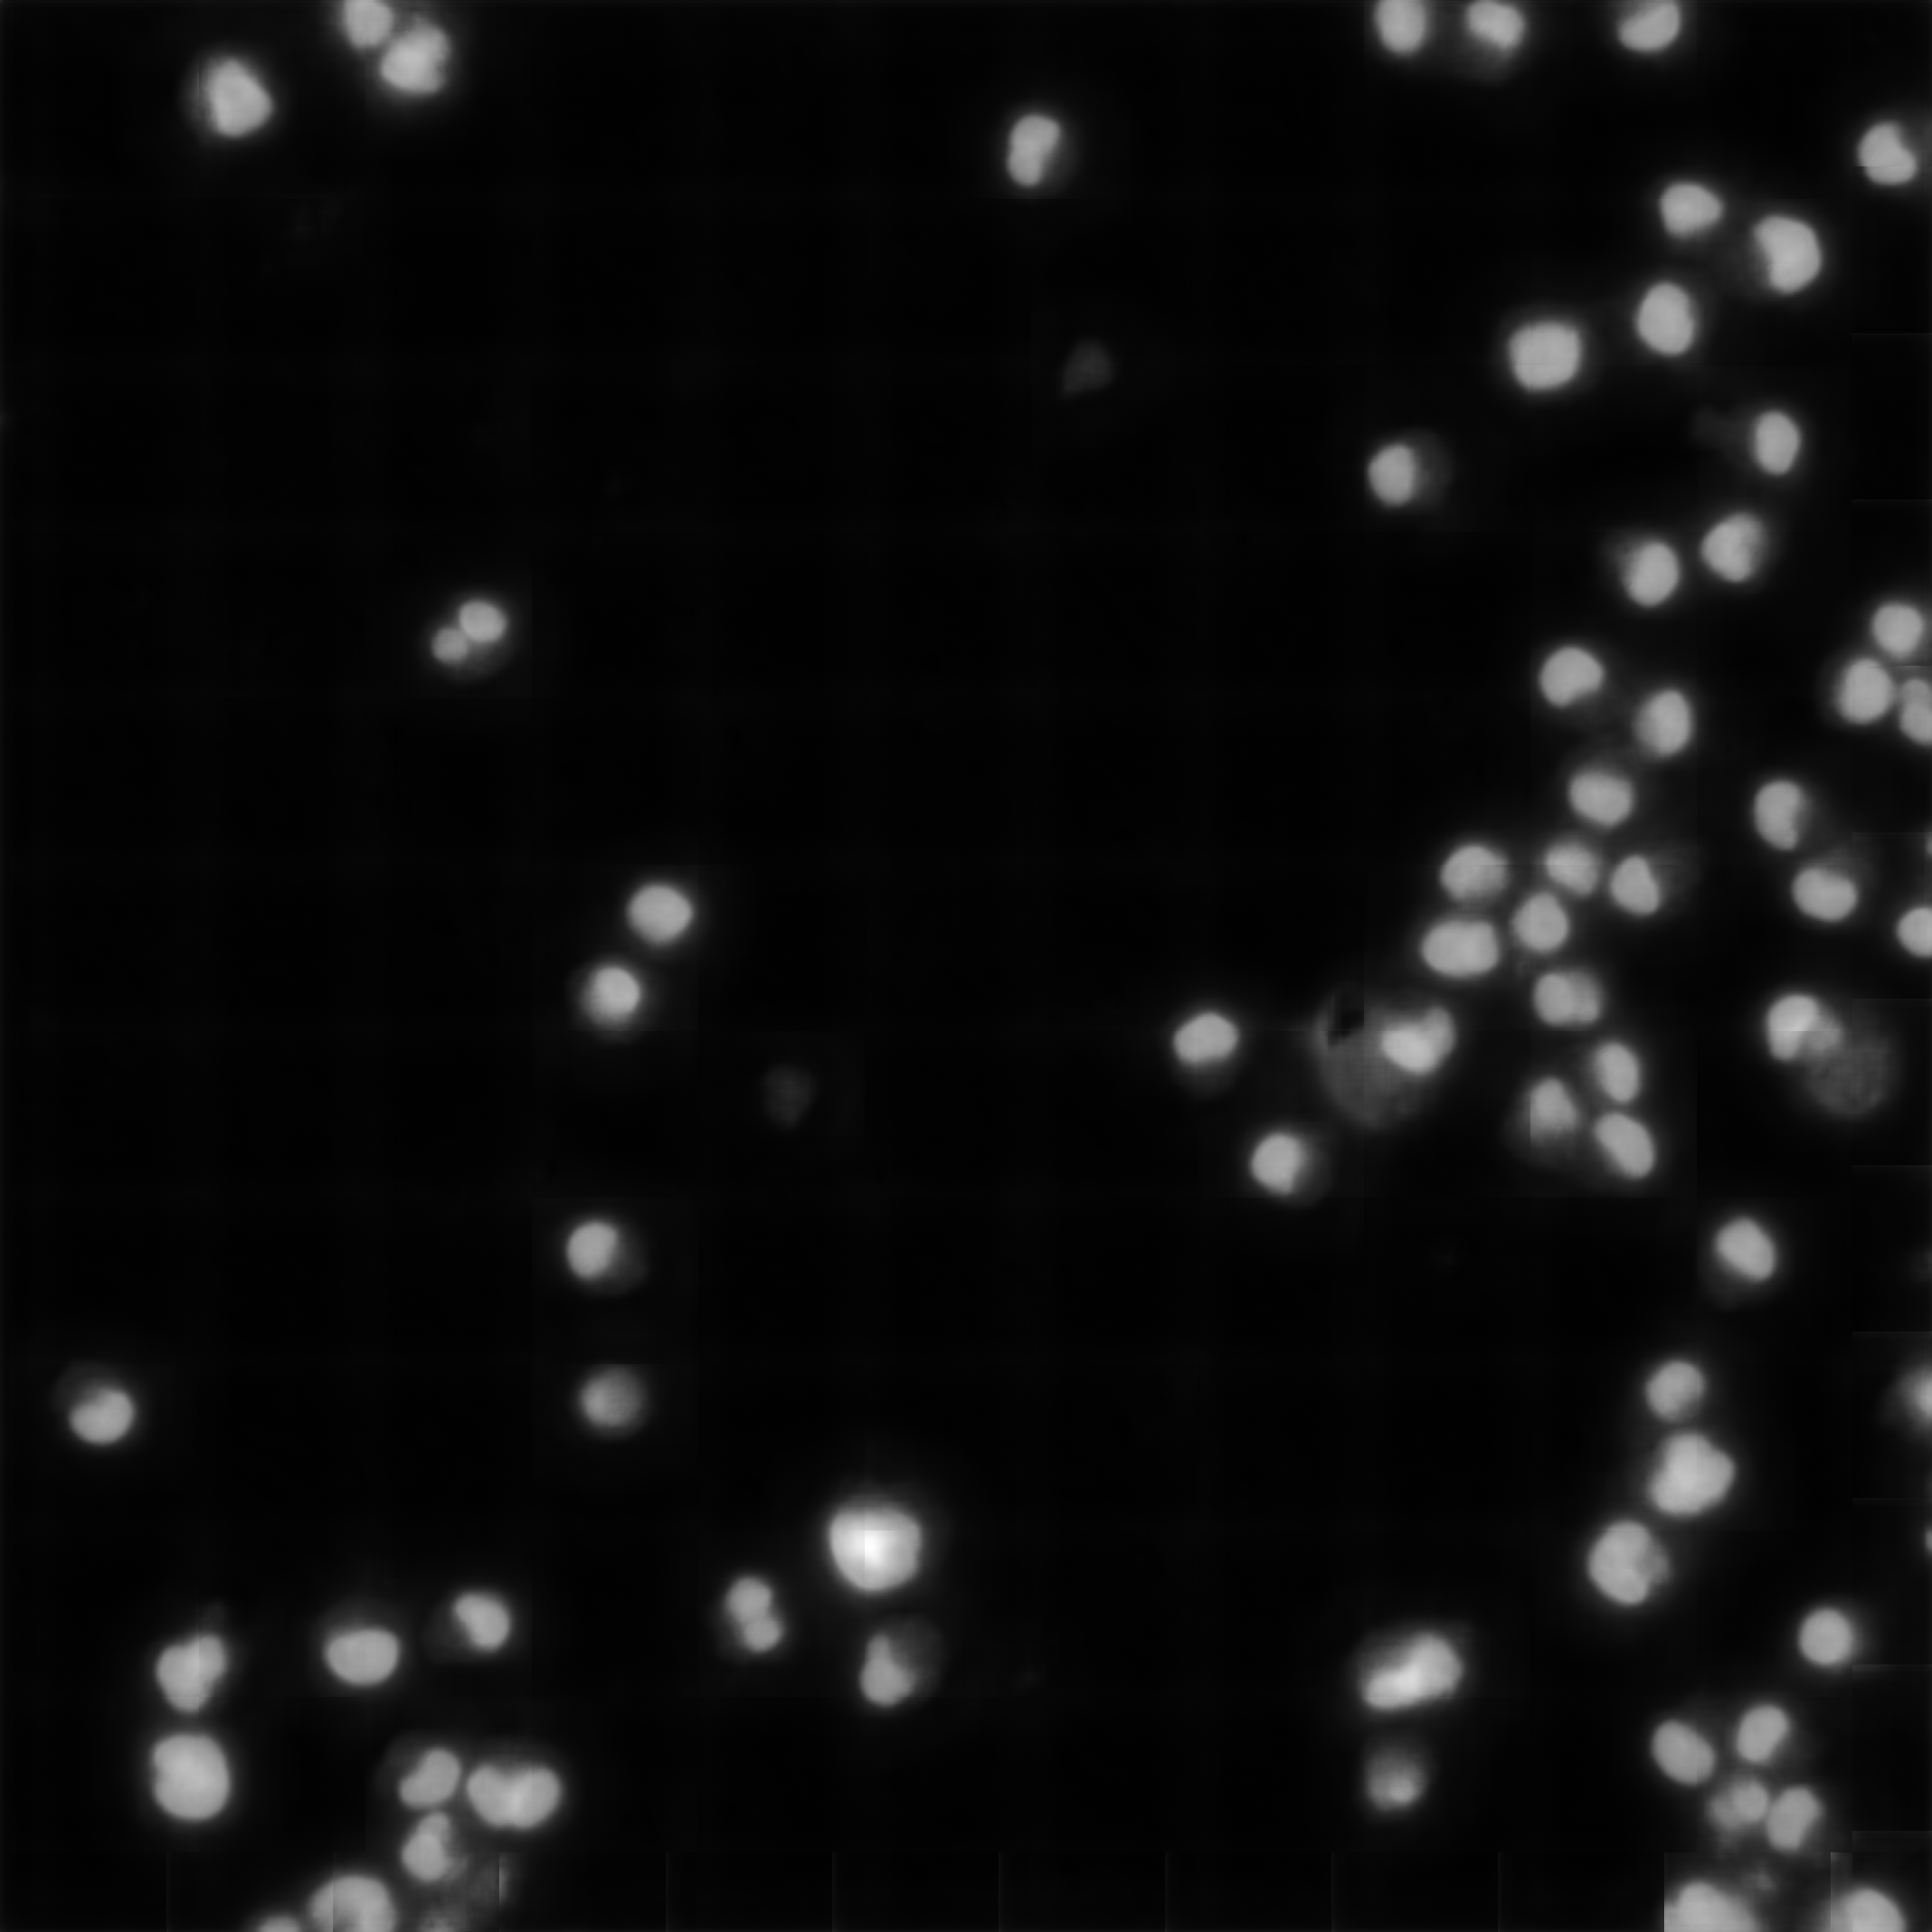
\includegraphics{bilder/lightning-conditions/lightning-1.png} & 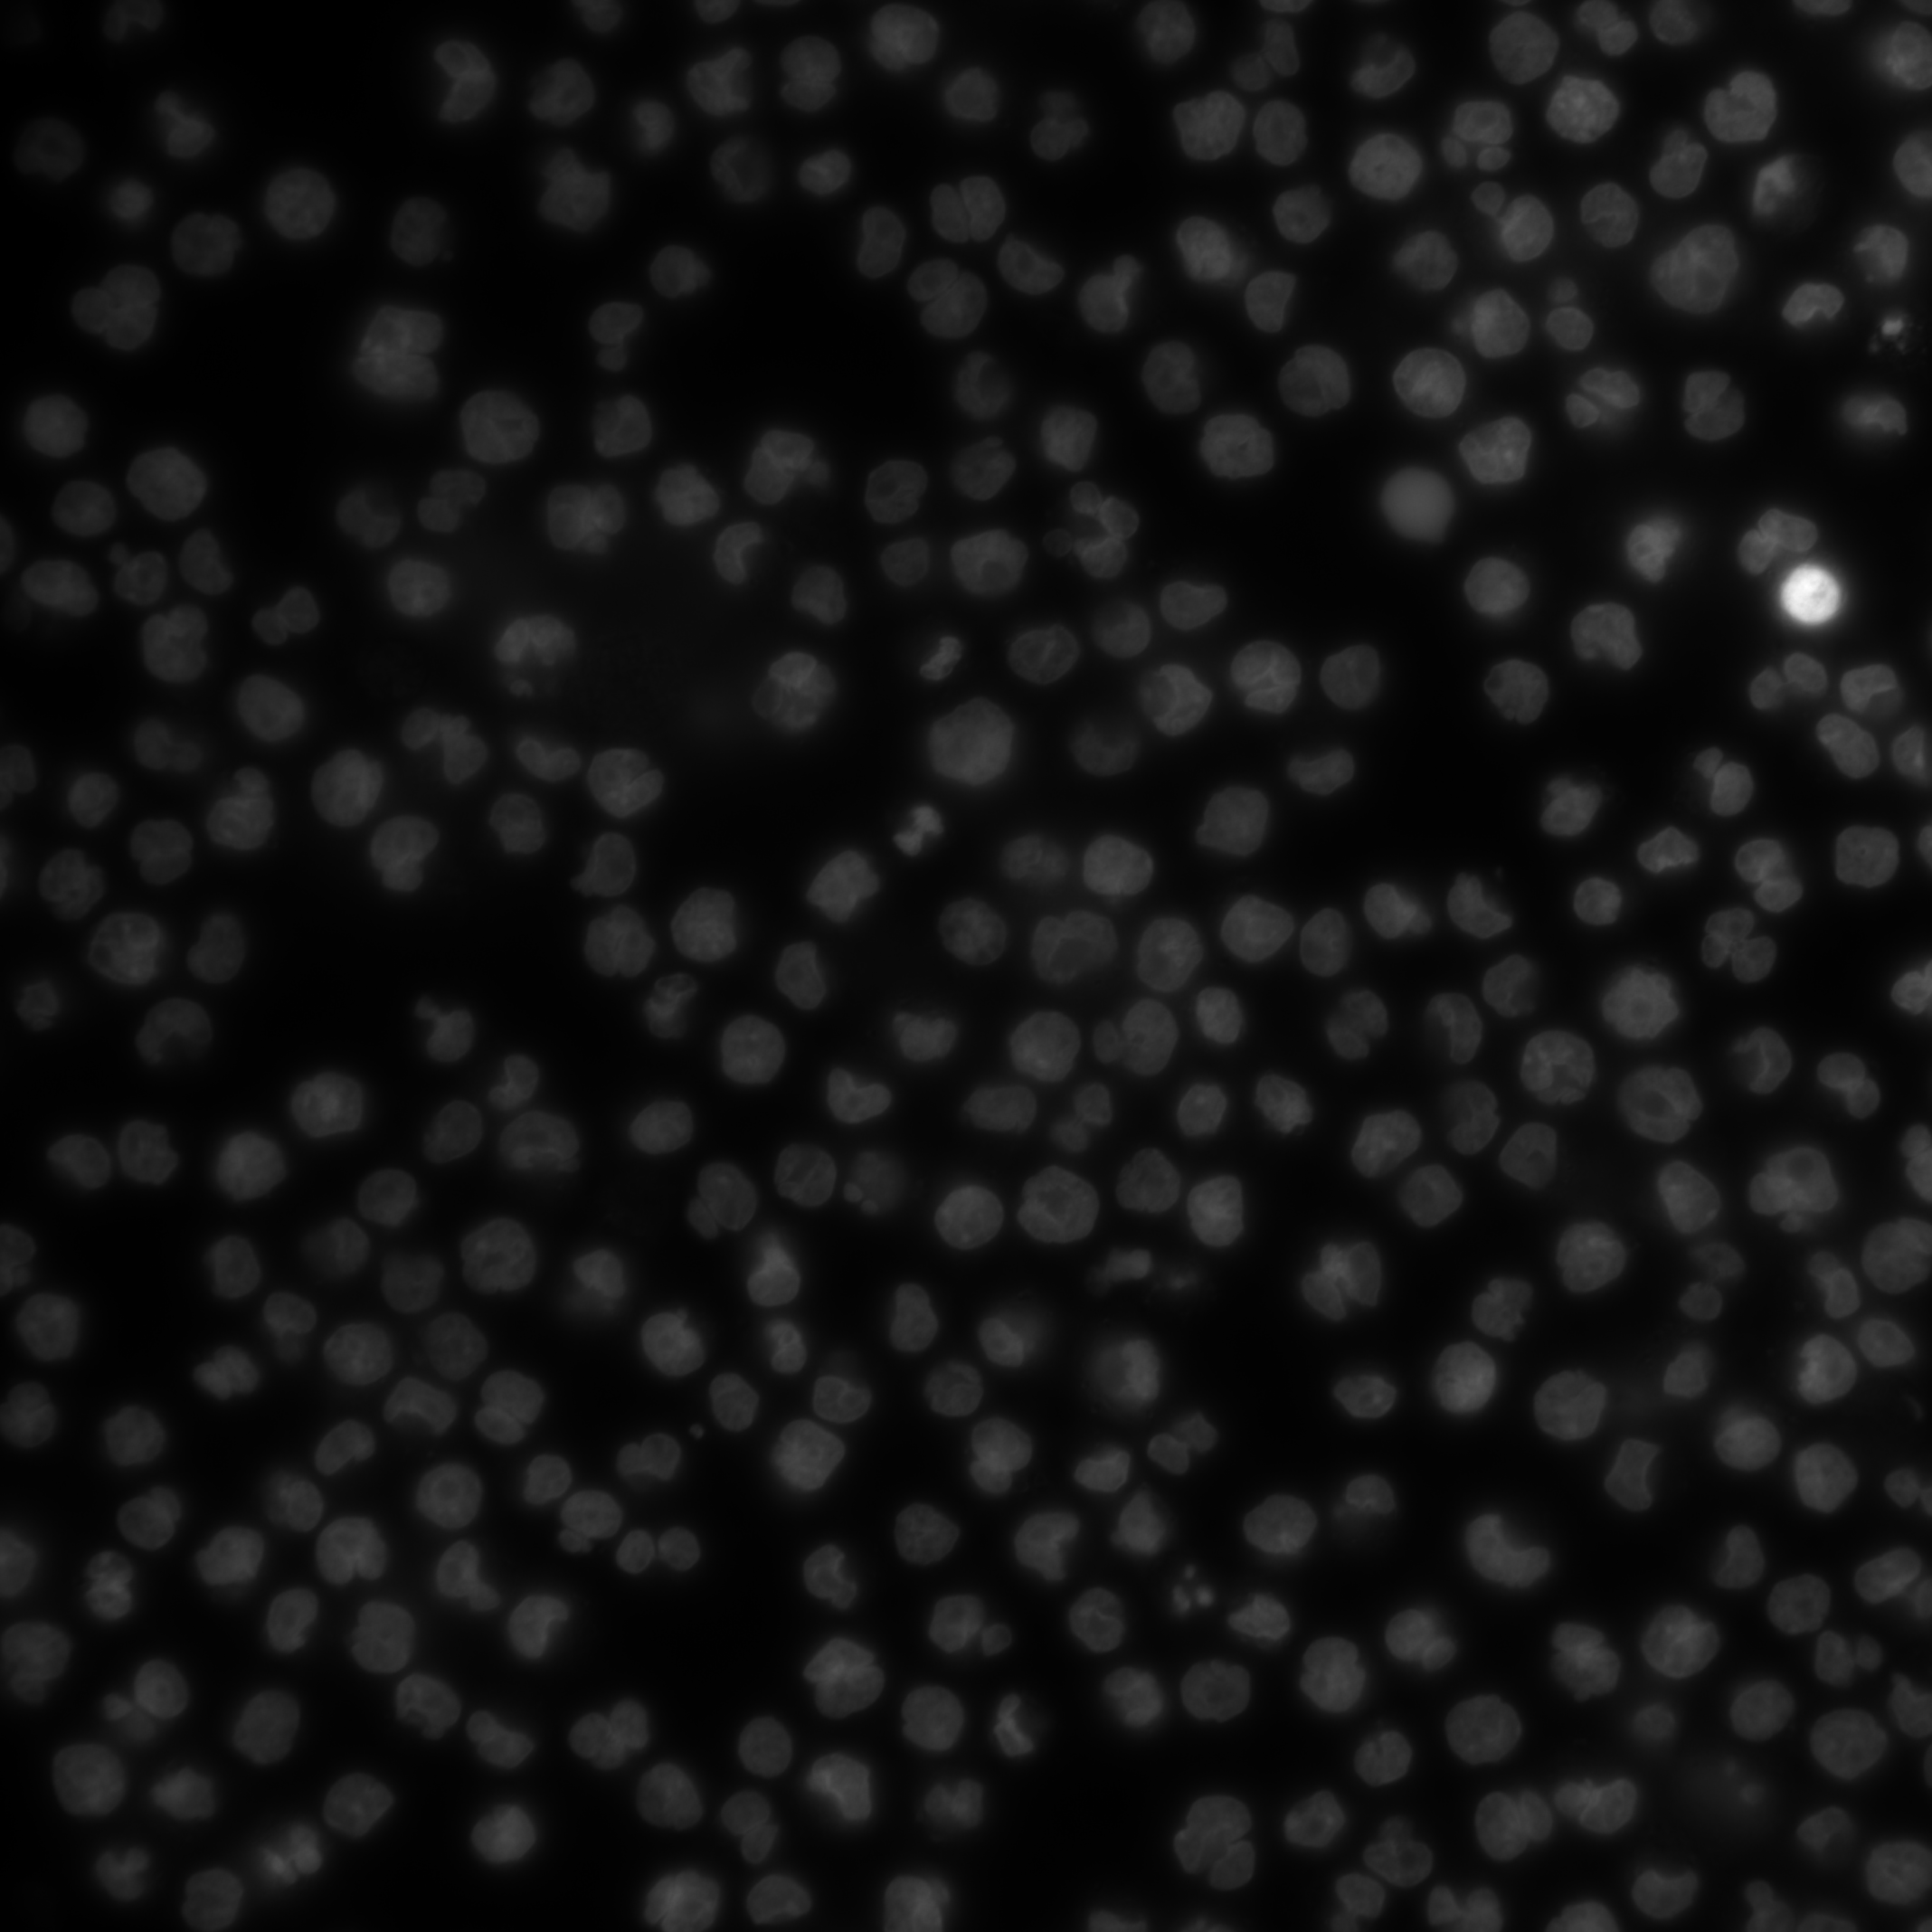
\includegraphics{bilder/lightning-conditions/lightning-2.png} &
            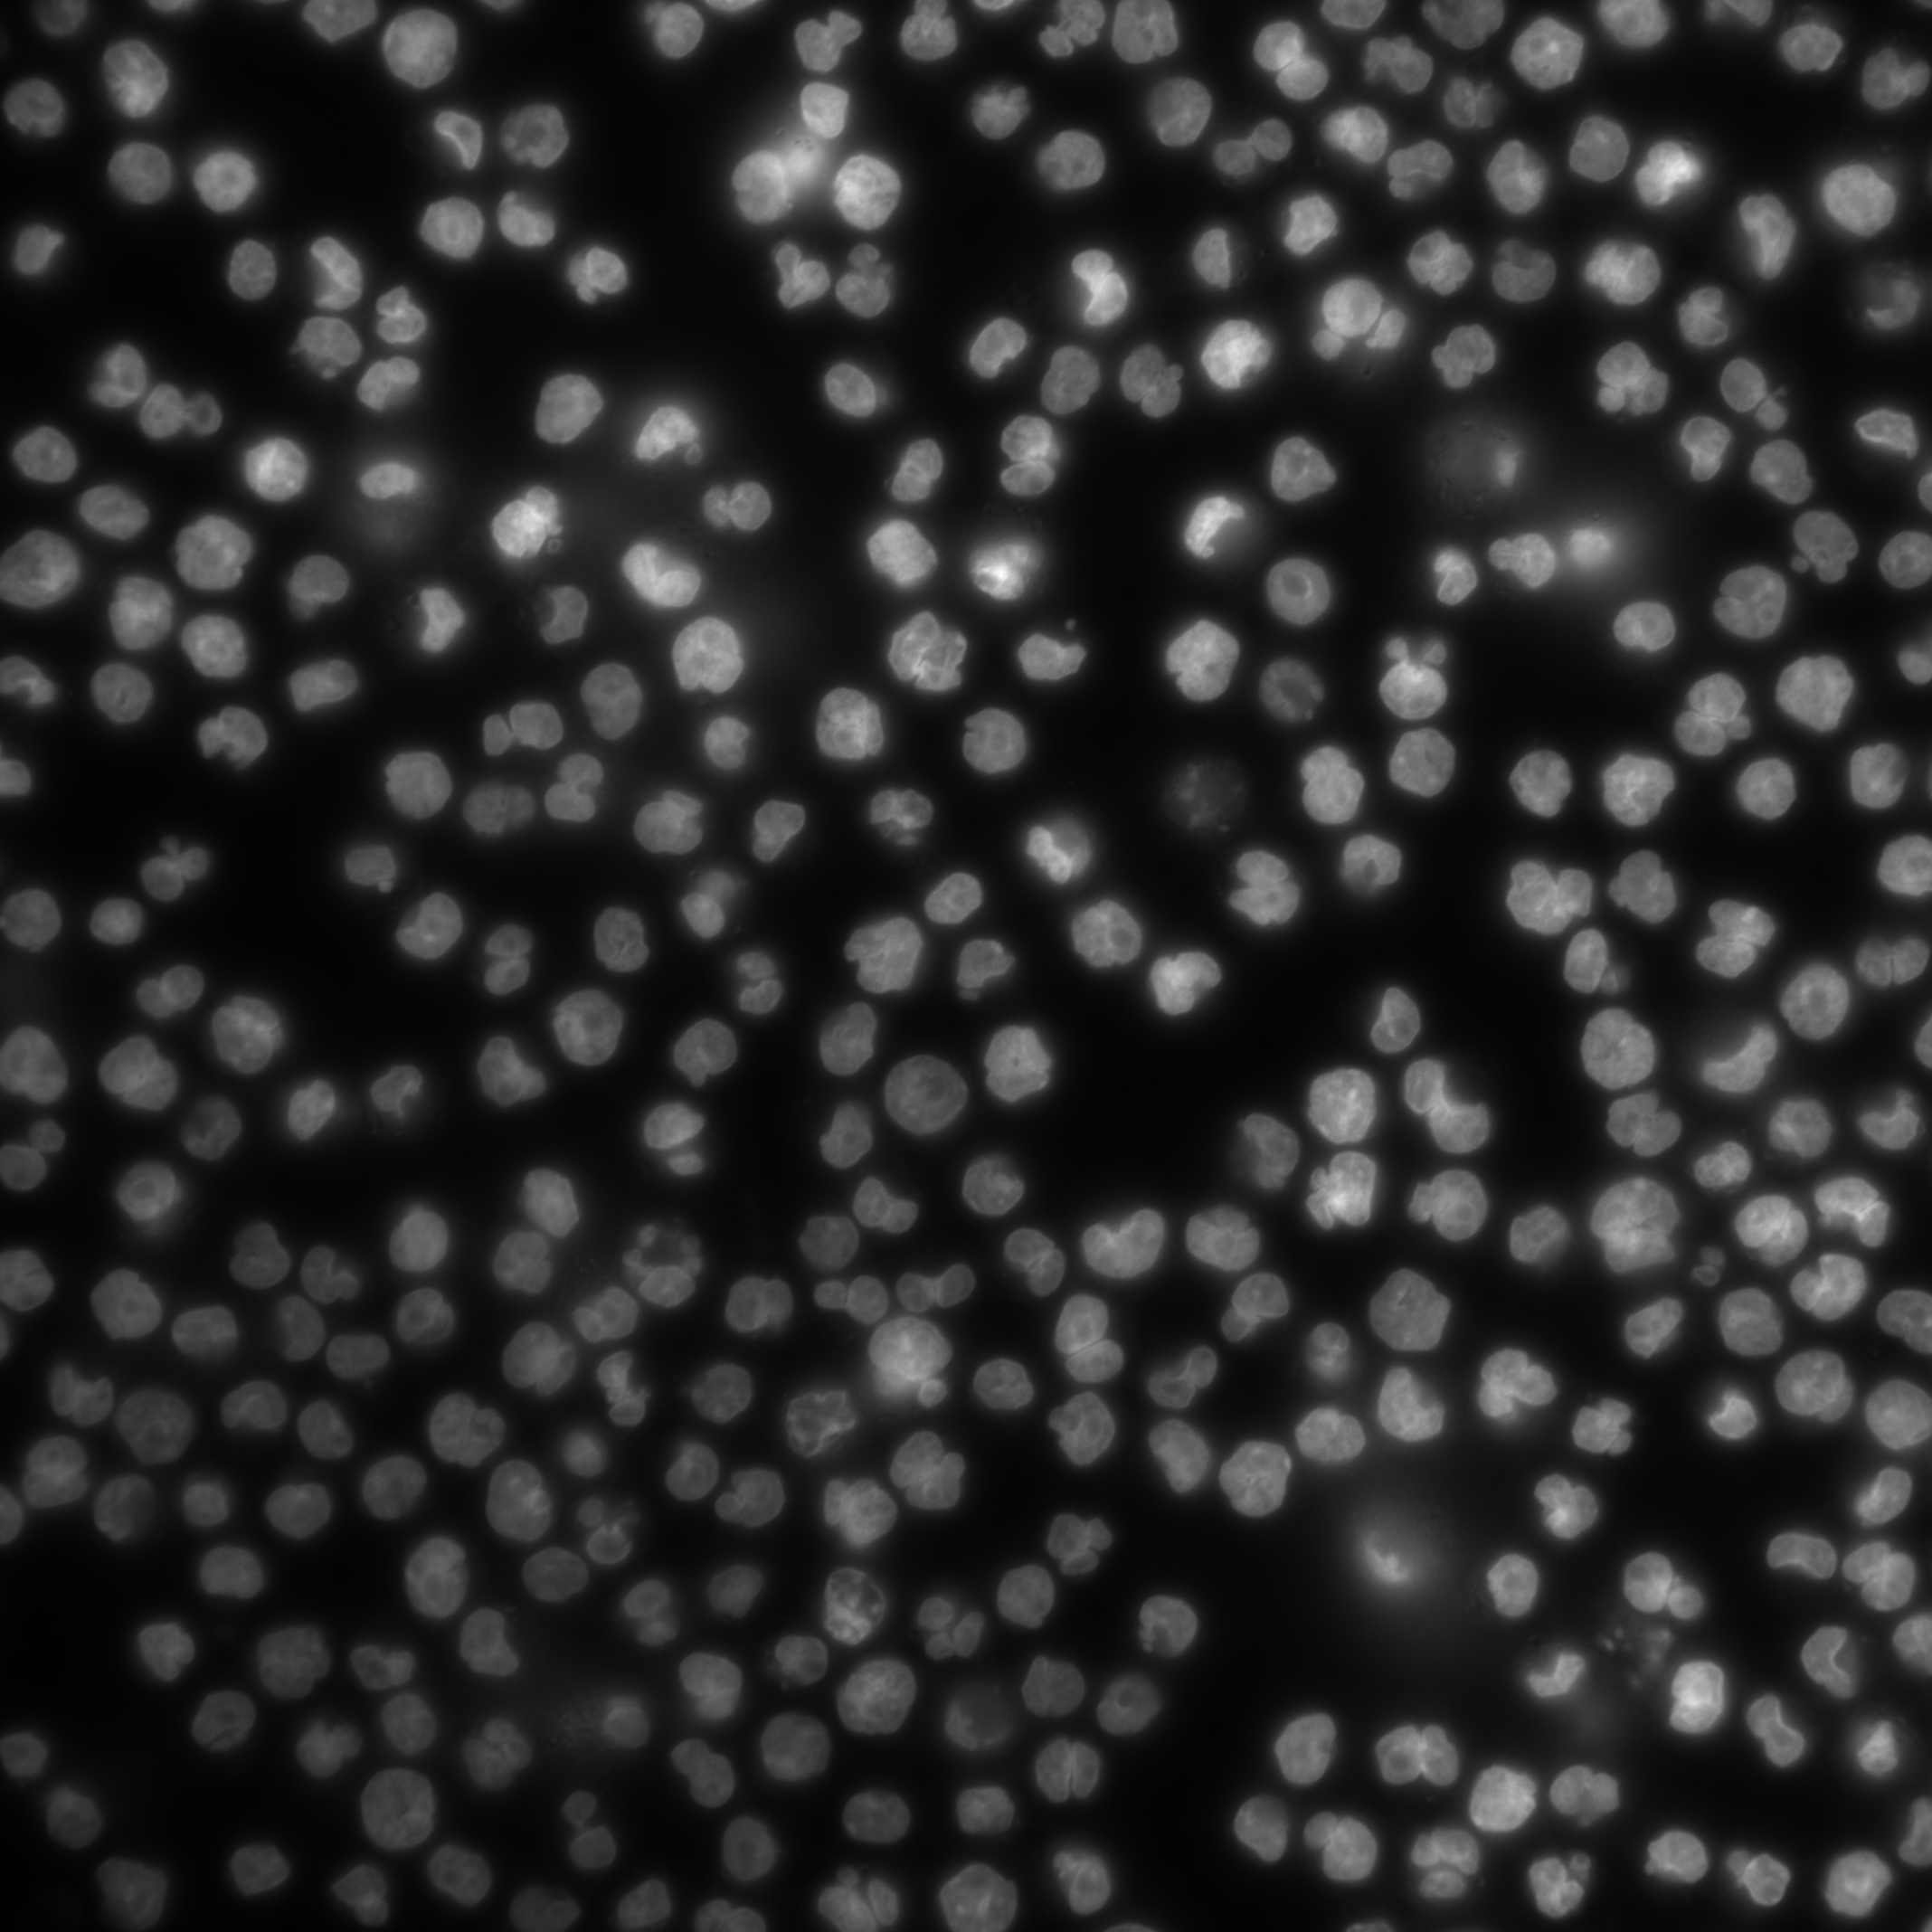
\includegraphics{bilder/lightning-conditions/lightning-3.png} & 
            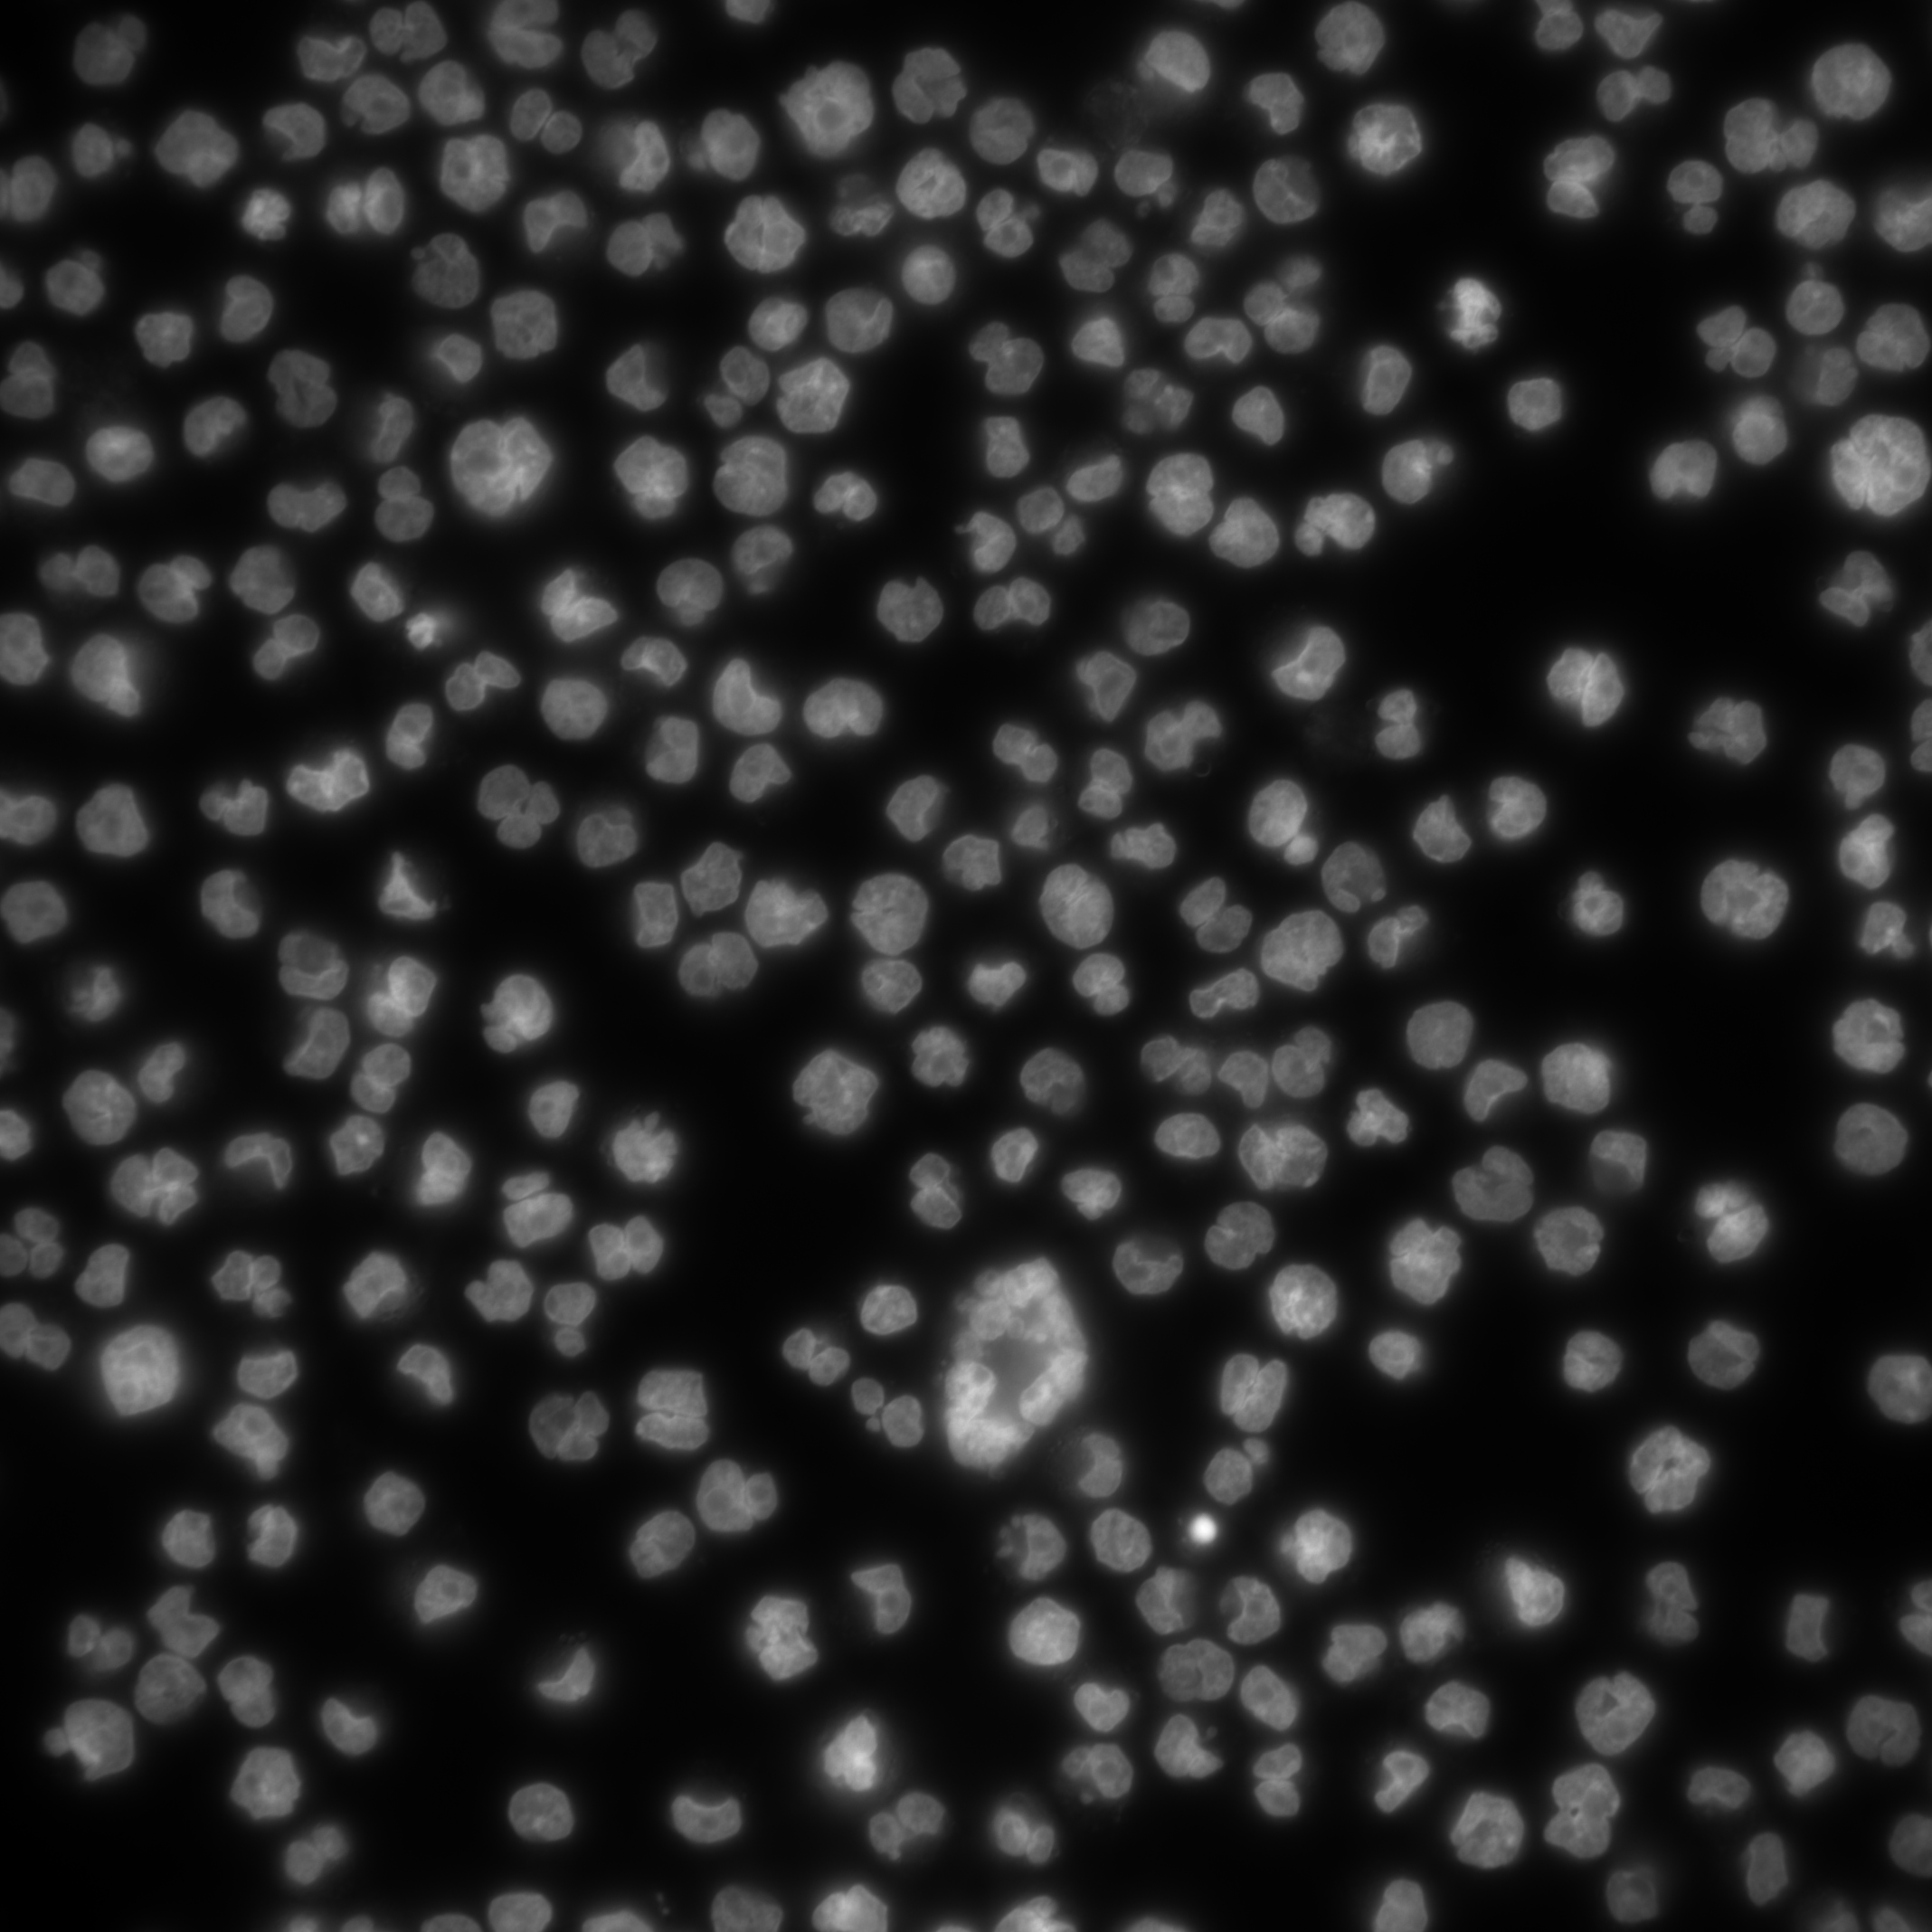
\includegraphics{bilder/lightning-conditions/lightning-4.png}
        \end{tabularx}
    \caption{Different lightning conditions}
    \label{fig:lightning_conditions}
\end{figure}

\begin{figure}[H]
    \centering
    \setkeys{Gin}{width=\linewidth}
    \centering
        \begin{tabularx}{\textwidth}{YY}
            \textbf{Original fluorescence} &
            \textbf{Segmentation} \\
            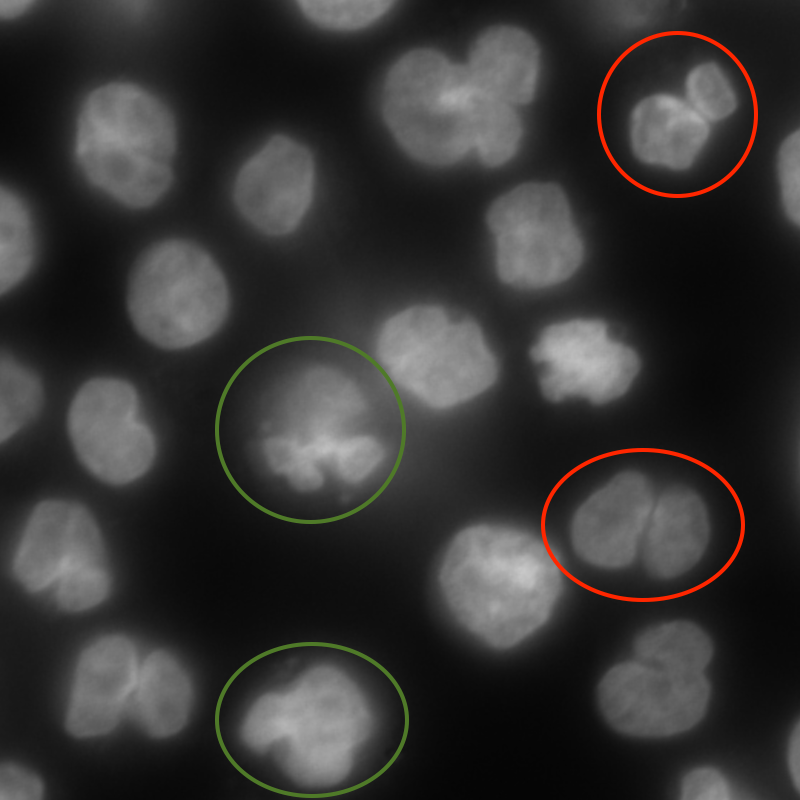
\includegraphics{bilder/close-located-cells/original.png} & 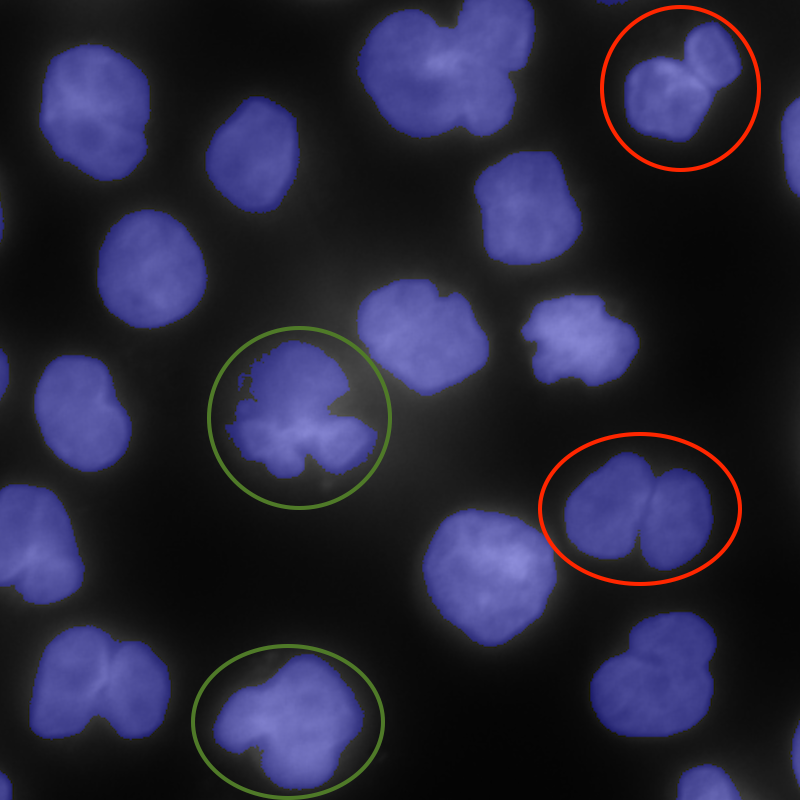
\includegraphics{bilder/close-located-cells/segmented.png}
        \end{tabularx}
    \caption{Closely located cells}
    \label{fig:closely-located-cells}
\end{figure}

Overall algorithm
\begin{figure}[H]
    \centering
    \setkeys{Gin}{width=\linewidth}
    \centering
        \begin{tabularx}{\textwidth}{YYYY}
            \textbf{Normalized input} &
            \textbf{Local threshold} &
            \textbf{Filled holes} &
            \textbf{Filtered regions} \\
            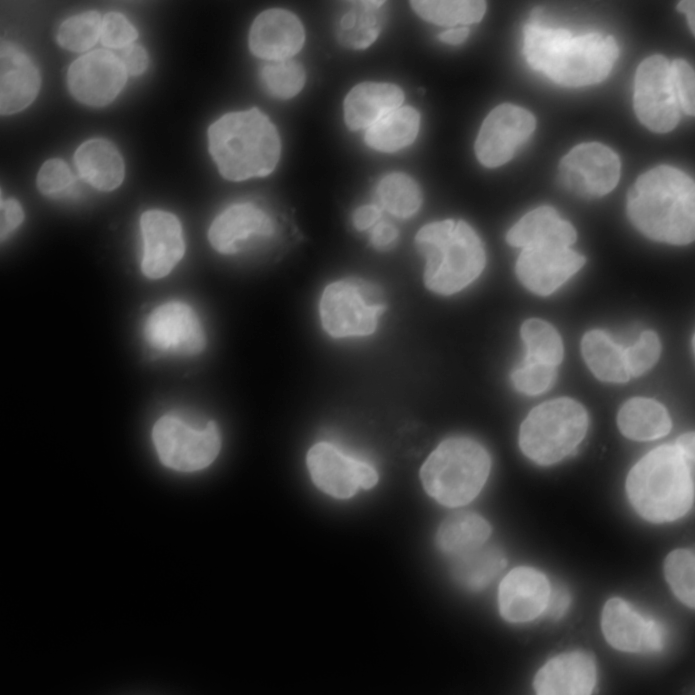
\includegraphics{bilder/segmentation/nuclei-mask/normalized.png} & 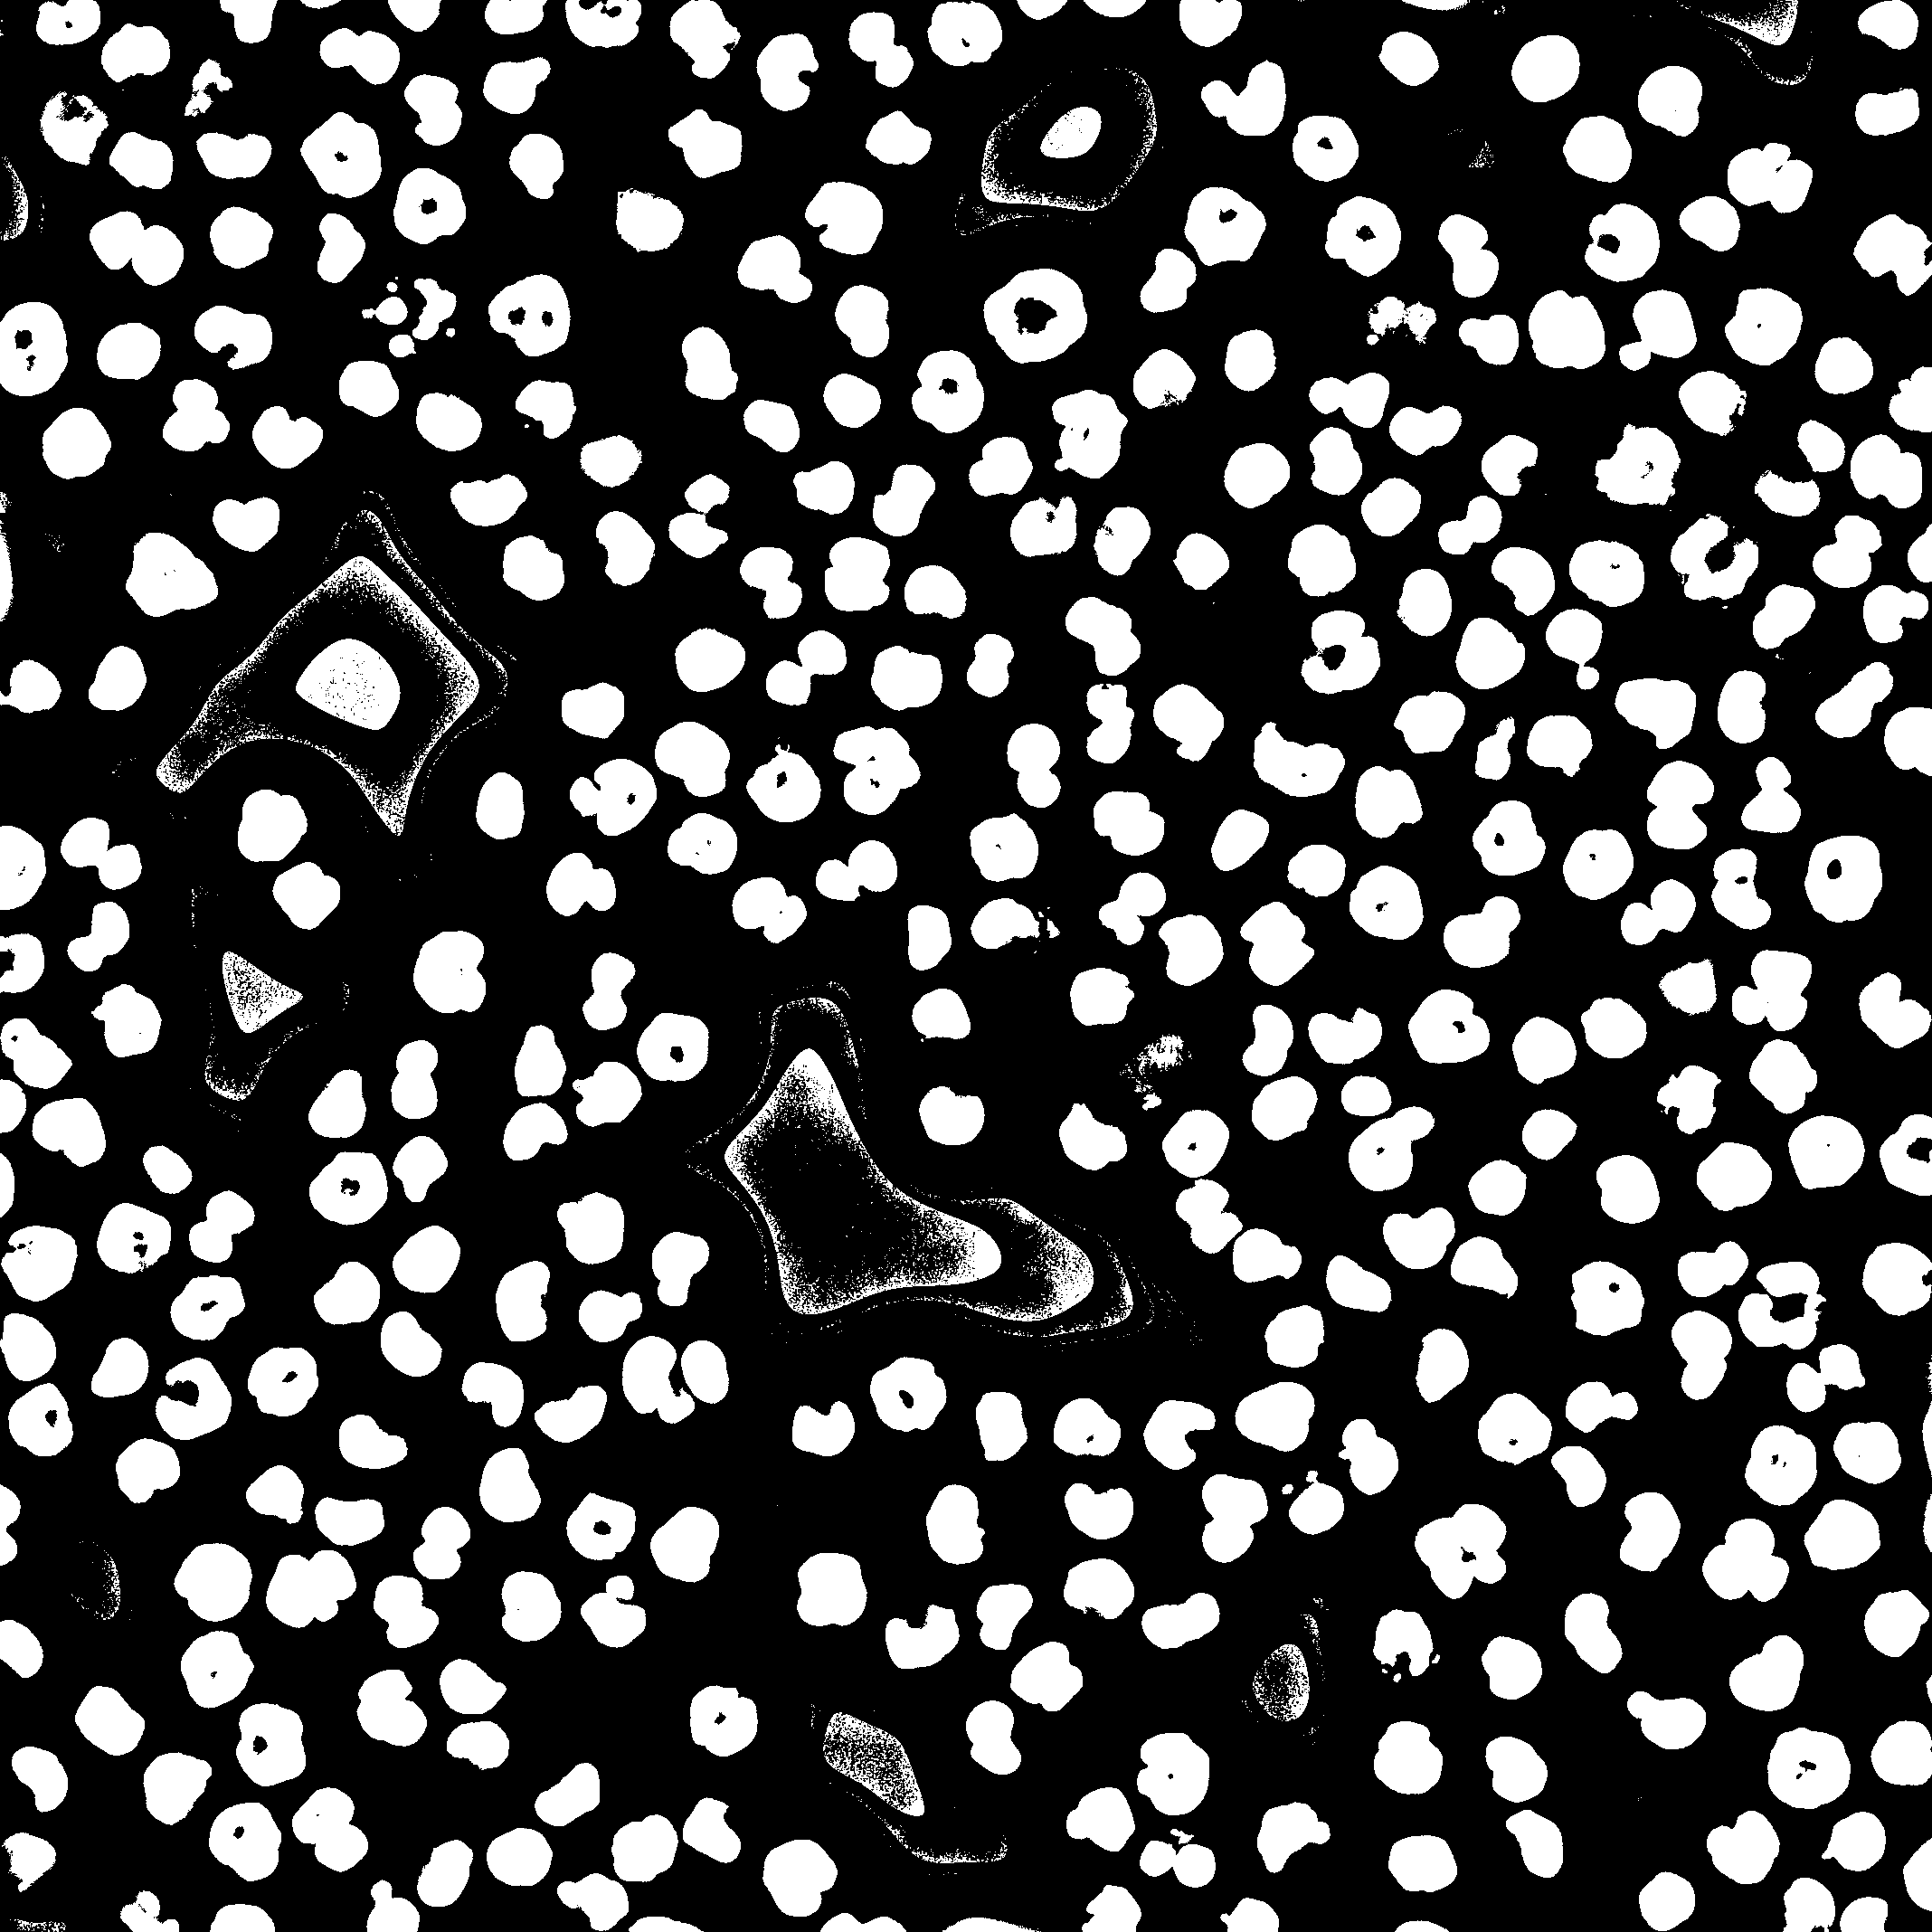
\includegraphics{bilder/segmentation/nuclei-mask/binary_local.png} &
            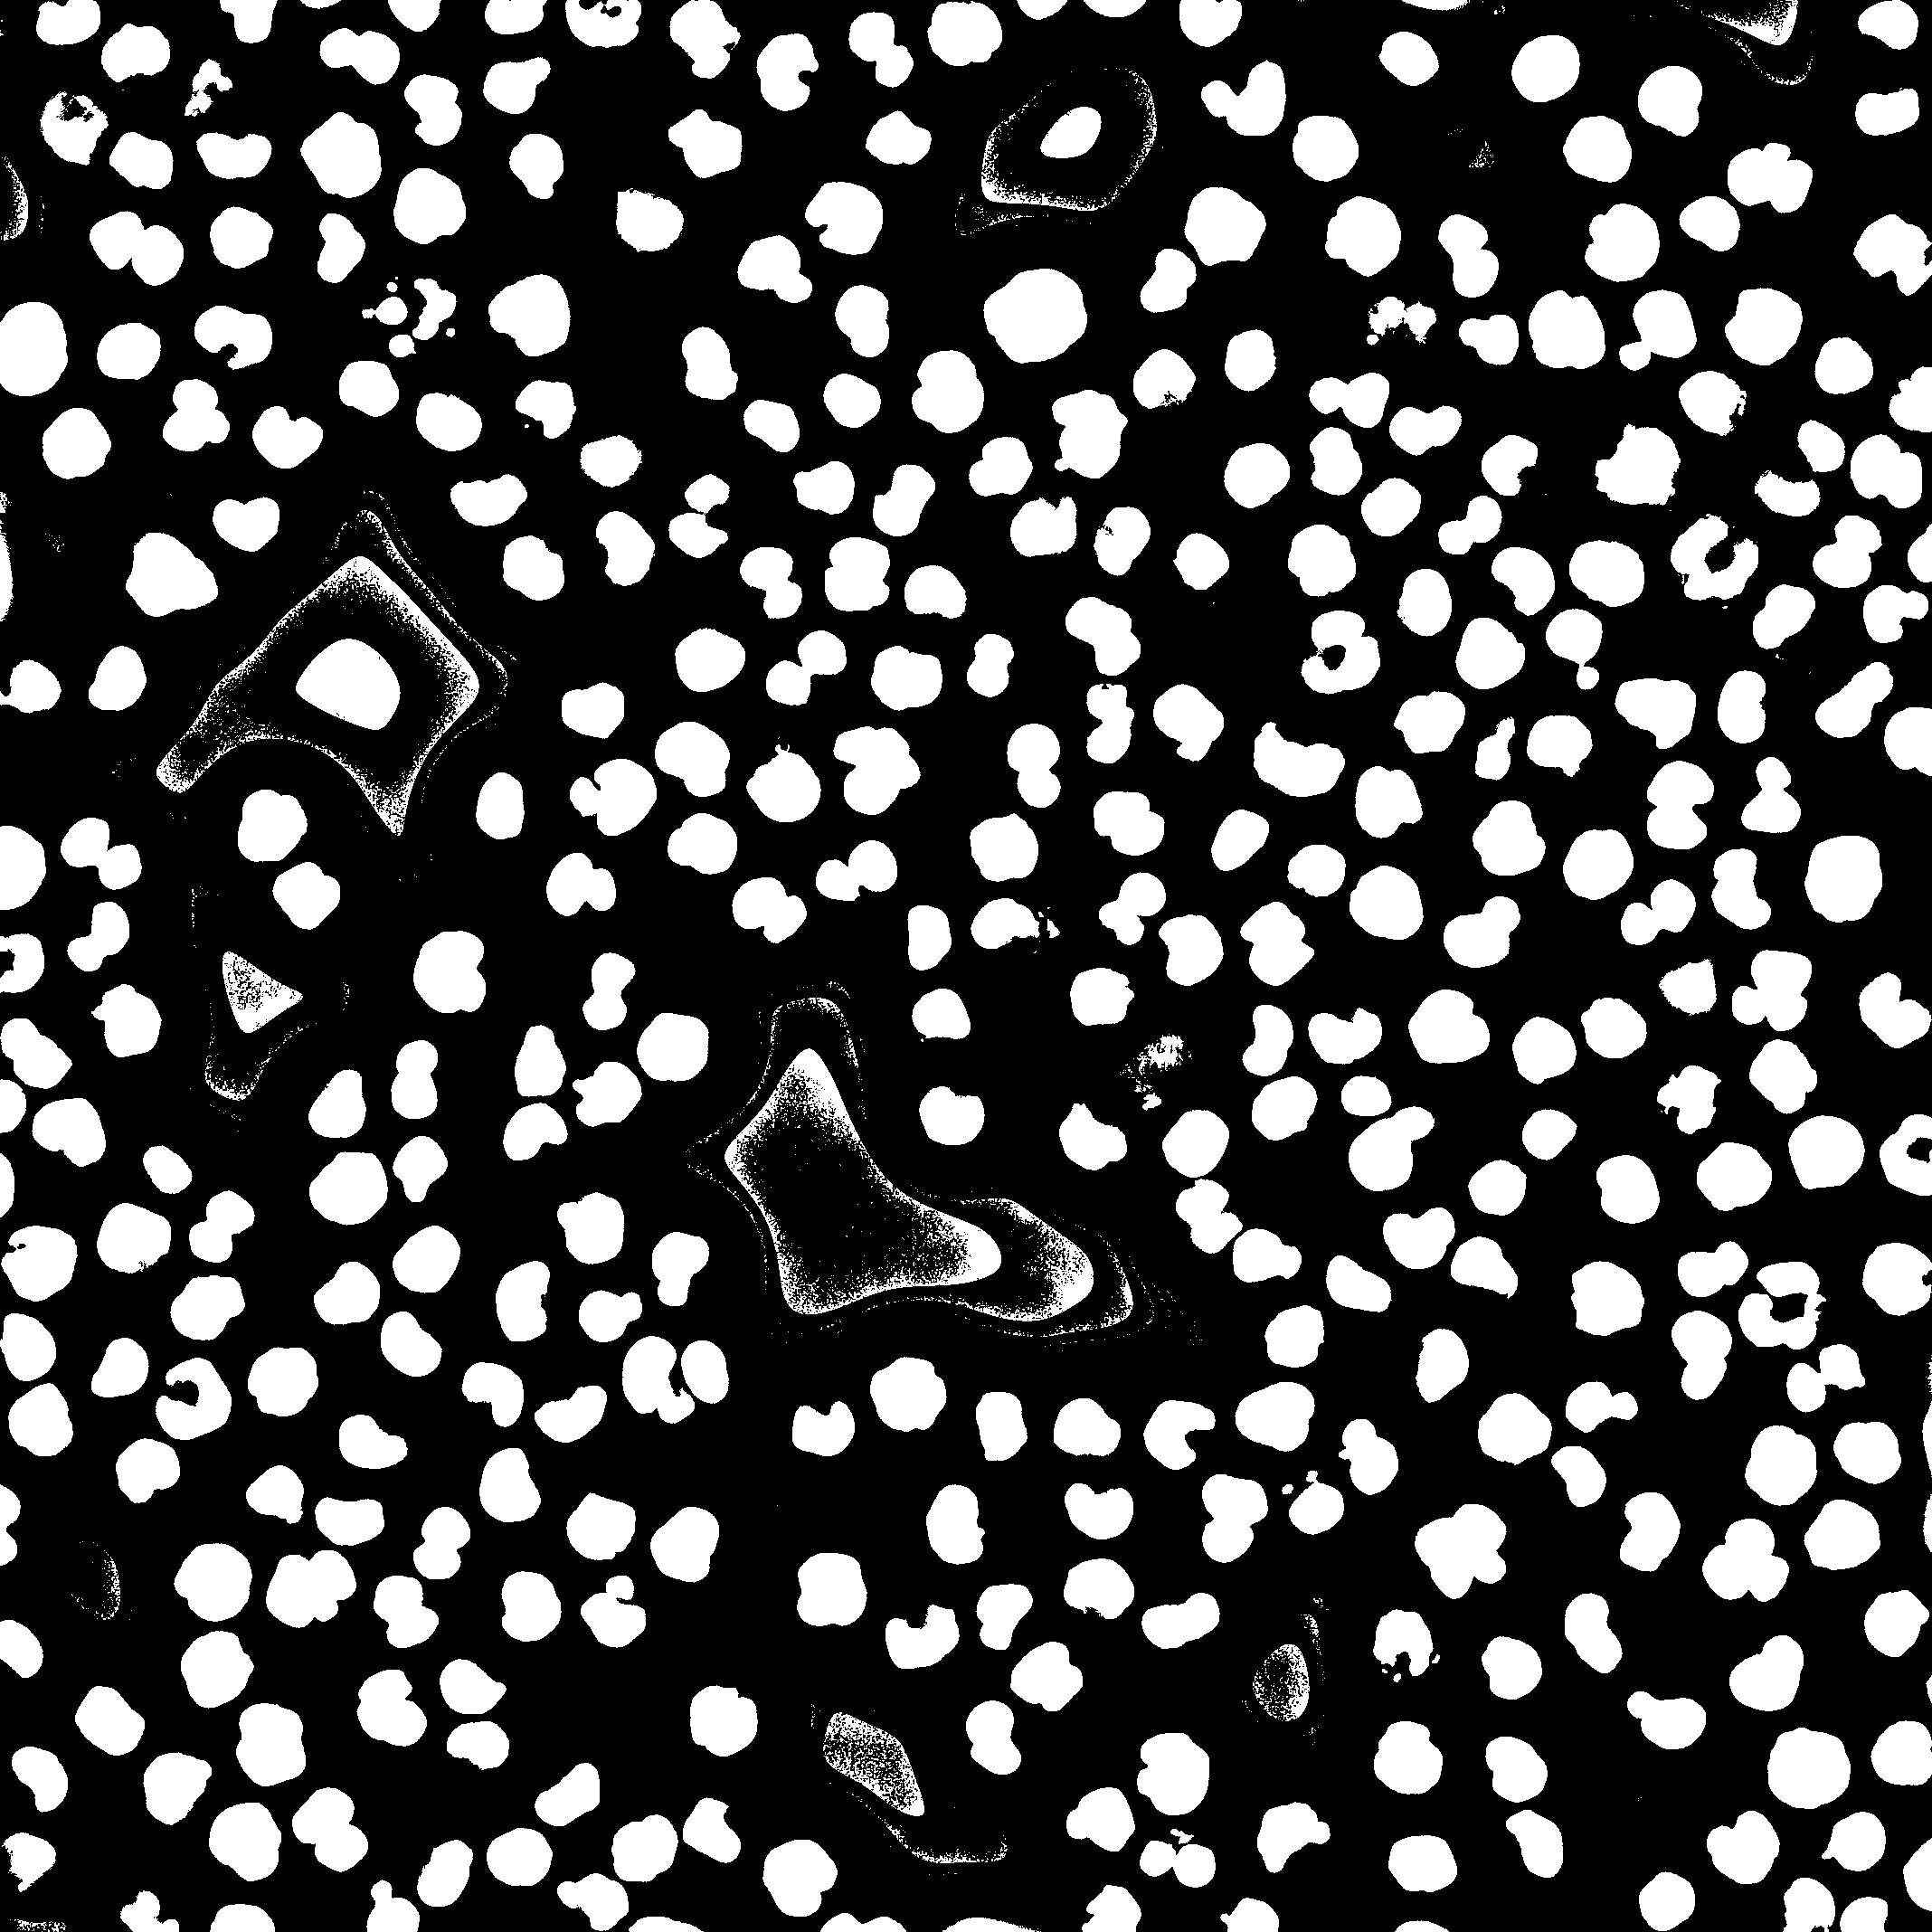
\includegraphics{bilder/segmentation/nuclei-mask/filled_holes.png} & 
            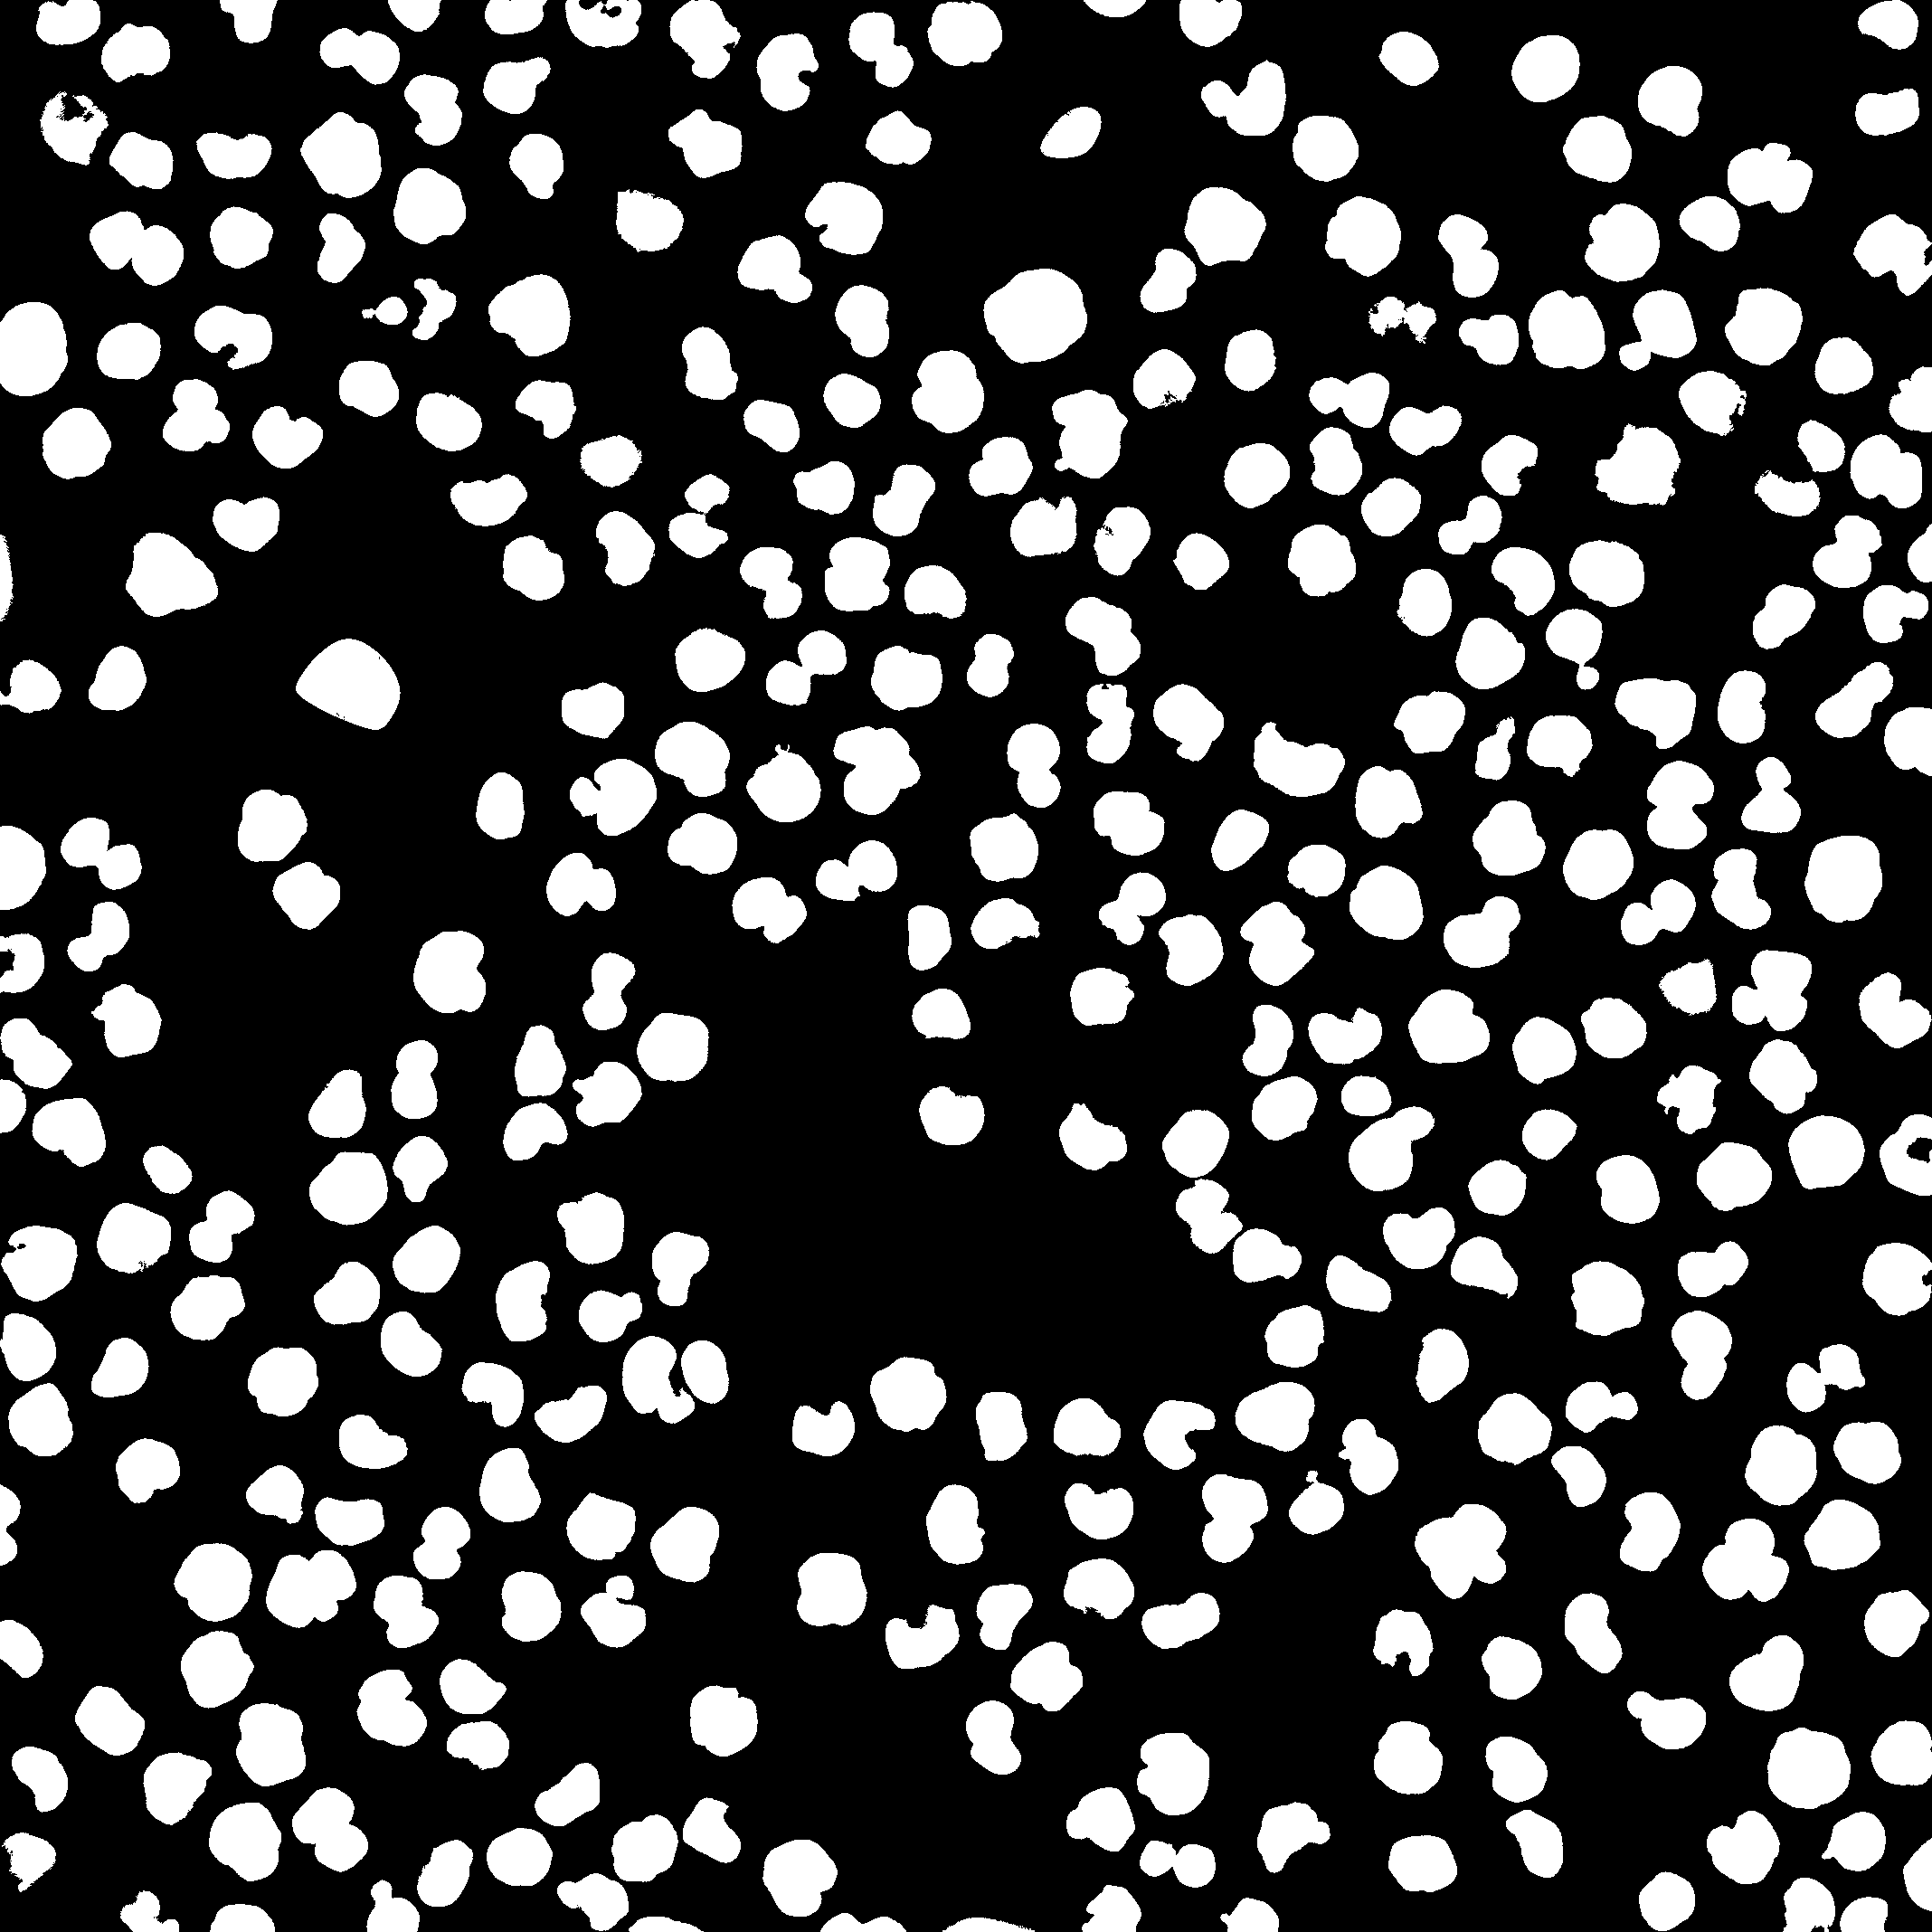
\includegraphics{bilder/segmentation/nuclei-mask/mask.png}
        \end{tabularx}
    \caption{Fluorescence segmentation}
    \label{fig:segmentation-nuclei-steps}
\end{figure}